\documentclass[11pt]{article}
% Shared preamble for the printable mini lessons (1.4 onward).
%   \documentclass[11pt]{article}
%   \input{../preamble}
% Build the key with:  pdflatex -jobname=<name>_KEY "\def\iskey{}\input{<name>}"
% Figures shared with the web page live in figures/Unit_X/<name>.tex and are
% pulled in with \fig{Unit_X/<name>}; the standalone package drops their own
% preamble, so their macros come from figures/preamble.tex, loaded here.
% Shared preamble for web figures.  Each figure is a standalone .tex that
% \input's this file; scripts/make-figures.sh turns it into an SVG.
\usepackage[T1]{fontenc}
\usepackage{helvet}
\renewcommand{\familydefault}{\sfdefault}
\usepackage{tikz}
\usetikzlibrary{decorations.pathreplacing}
% axis numbers in the text font, not math italic
\pgfkeys{/pgf/number format/.cd,assume math mode=true,1000 sep={}}

% dot plot: \dotplot{min}{max}{value/count,...}{axis label}
\newcommand{\dotplot}[4]{%
\begin{tikzpicture}[x=0.9cm,y=0.33cm]
  \draw[thick] (#1-0.5,0) -- (#2+0.5,0);
  \foreach \t in {#1,...,#2} {\draw (\t,0.25) -- (\t,-0.25) node[below] {\t};}
  \foreach \v/\c in {#3} {\ifnum\c>0 \foreach \k in {1,...,\c} {\fill (\v,\k*1.15) circle (0.16cm);}\fi}
  \node at ({(#1+#2)/2},-2.3) {#4};
\end{tikzpicture}}

% shape sketch histogram (12 bins): \shapehist{heights}{label}
\newcommand{\shapehist}[2]{%
  \foreach \h [count=\i from 0] in {#1} \draw[fill=gray!30] (\i,0) rectangle (\i+1,\h);
  \draw (-0.3,0) -- (12.3,0);
  \node[font=\bfseries] at (6,-2.6) {#2};}
\newcommand{\meanmark}[1]{\fill (#1,0) -- ++(-0.3,-0.75) -- ++(0.6,0) -- cycle;}
\newcommand{\medmark}[2]{\draw[very thick,dashed] (#1,0) -- (#1,#2);}

% number line with minor ticks: \nline{min}{max}{label step}{axis label}
\newcommand{\nline}[4]{%
  \draw[thick] (#1-0.5,0) -- (#2+0.5,0);
  \foreach \t in {#1,...,#2} \draw (\t,0.12) -- (\t,-0.12);
  \pgfmathtruncatemacro{\nxt}{#1+#3}
  \foreach \t in {#1,\nxt,...,#2} \draw (\t,0.2) -- (\t,-0.2) node[below] {\t};
  \node at ({(#1+#2)/2},-0.95) {#4};}
% box plot above the line: \bplot{min}{Q1}{med}{Q3}{max}
\newcommand{\bplot}[5]{%
  \draw[thick] (#1,1.0) -- (#2,1.0);
  \draw[thick] (#4,1.0) -- (#5,1.0);
  \draw[thick] (#1,0.75) -- (#1,1.25);
  \draw[thick] (#5,0.75) -- (#5,1.25);
  \draw[thick,fill=gray!20] (#2,0.55) rectangle (#4,1.45);
  \draw[very thick] (#3,0.55) -- (#3,1.45);}

% ---- added for 1.4 onward ----
% axis on y=0: \axis{min}{max}{label step}{tick step}{axis label}
\newcommand{\axis}[5]{%
  \draw[thick] (#1,0) -- (#2,0);
  \pgfmathsetmacro{\axT}{#1+#4}\foreach \t in {#1,\axT,...,#2} \draw (\t,0.1) -- (\t,-0.1);
  \pgfmathsetmacro{\axL}{#1+#3}\foreach \t in {#1,\axL,...,#2}
    \draw (\t,0.18) -- (\t,-0.18) node[below] {\pgfmathprintnumber{\t}};
  \node at ({(#1+#2)/2},-0.95) {#5};}
% box plot centred at height y: \bplotat{y}{min}{Q1}{med}{Q3}{max}
\newcommand{\bplotat}[6]{%
  \draw[thick] (#2,#1) -- (#3,#1);
  \draw[thick] (#5,#1) -- (#6,#1);
  \draw[thick] (#2,#1-0.22) -- (#2,#1+0.22);
  \draw[thick] (#6,#1-0.22) -- (#6,#1+0.22);
  \draw[thick,fill=gray!20] (#3,#1-0.42) rectangle (#5,#1+0.42);
  \draw[very thick] (#4,#1-0.42) -- (#4,#1+0.42);}
% an outlier dot: \outlier{x}{y}
\newcommand{\outlier}[2]{\fill (#1,#2) circle (2.4pt);}

\usepackage[margin=0.75in]{geometry}
\usepackage{array}
\usepackage{enumitem}
\usepackage{amsmath}
\usepackage[helvet]{sfmath}  % math in the same sans font as the text
\usepackage{standalone}
\pagestyle{empty}
\setlength{\parindent}{0pt}
\setlist[enumerate,1]{leftmargin=1.5em,itemsep=1em}
\setlist[enumerate,2]{label=(\alph*),leftmargin=2em,itemsep=2.2em}

\newif\ifkey
\ifdefined\iskey \keytrue \fi
\colorlet{keyred}{red!75!black}
\newcommand{\ans}[1]{\ifkey\leavevmode{\color{keyred}#1}\fi}
% vertical work space on the student copy, less on the key
\newcommand{\work}[1]{\ifkey\vspace{0.6em}\else\vspace{#1}\fi}
\newcommand{\fig}[1]{\input{../../figures/#1}}
% Title line: \lessontitle{Quartiles, IQR, and Box Plots}
\newcommand{\lessontitle}[1]{{\Large\bfseries #1\ifkey\ \textcolor{keyred}{KEY}\fi}\hfill Name \underline{\hspace{2in}}\par\vspace{0.6em}}
\newcommand{\partner}{\par\vspace{0.4em}Work with a partner. Compare answers when you finish each problem.\par}

% Unit quiz: two questions per mini lesson, each headed by the lesson's
% objective.  The key keeps every box the same height as the student copy,
% so key page N lines up with quiz page N.
\newcommand{\lessonhead}[1]{\par\vspace{0.6em}{\large\bfseries #1}\par\vspace{0.25em}\hrule\vspace{0.6em}}
\newcommand{\goal}[1]{\textbf{#1}\par\vspace{0.35em}}
% answer box: same height on both copies, answer printed only on the key
\newcommand{\abox}[2]{\par\begin{minipage}[t][#1][t]{\linewidth}\raggedright\vspace{0.2em}\ans{#2}\end{minipage}\par}
% circled choices: \opt{A} prints plain; \optans{B} is circled in red on the key
\newcommand{\opt}[1]{\tikz[baseline=(c.base)]\node[rounded corners=0.6em,inner sep=2.5pt](c){#1};}
\newcommand{\optans}[1]{\ifkey\tikz[baseline=(c.base)]\node[rounded corners=0.6em,inner sep=2.5pt,draw=keyred,thick,text=keyred](c){#1};\else\opt{#1}\fi}
% blank probability bar graph (\probbars with every bar at height 0);
% the key draws the bars in red: \blankbars{xmax}{x/0,...}{ymax}{x label}{x/p,...}
\newcommand{\blankbars}[5]{%
  \def\pbmax{#1}\probbars{#2}{#3}{0.1}{#4}%
  \ifkey\foreach \x/\p in {#5} \draw[keyred,thick,fill=red!12] (\x-0.35,0) rectangle (\x+0.35,\p);\fi}
\setlist[enumerate,2]{label=(\alph*),leftmargin=2em,itemsep=0.3em}
\setlist[enumerate,1]{leftmargin=1.5em,itemsep=1em}
\raggedright\hyphenpenalty=10000\exhyphenpenalty=10000

\begin{document}

\lessontitle{Unit 7 Quiz: Probability Distributions}

Show your work.

% ======================================================================
\lessonhead{7.1 - Probability Distributions}
\begin{enumerate}

\item \goal{I check if a probability distribution is valid, and I draw it as a graph.}
\begin{enumerate}
  \item Is this table a valid probability distribution? Explain.

  \vspace{0.3em}
  \begin{minipage}[t]{0.38\linewidth}\vspace{0pt}
  \renewcommand{\arraystretch}{1.4}
  \begin{tabular}{|c|c|c|c|c|}\hline $x$ & 1 & 2 & 3 & 4\\ \hline $P(x)$ & 0.2 & 0.5 & 0.4 & $-0.1$\\ \hline\end{tabular}
  \end{minipage}\hfill
  \begin{minipage}[t][3.4em][t]{0.6\linewidth}\vspace{0pt}\raggedright
  \ans{Not valid. The probabilities add to 1, but $-0.1$ is less than 0. A probability cannot be negative.}
  \end{minipage}
\end{enumerate}

\vspace{0.4em}
\begin{minipage}[t]{0.5\linewidth}\vspace{0pt}\raggedright
Let $X$ = the number of times the school bus is late in one week.
\end{minipage}\hfill
\begin{minipage}[t]{0.46\linewidth}\vspace{0pt}\raggedleft
\renewcommand{\arraystretch}{1.4}
\begin{tabular}{|c|c|c|c|c|c|}\hline
$x$ & 0 & 1 & 2 & 3 & 4\\ \hline
$P(x)$ & 0.35 & 0.30 & \;?\; & 0.10 & 0.05\\ \hline
\end{tabular}
\end{minipage}

\vspace{0.6em}
\begin{minipage}[t]{0.47\linewidth}\vspace{0pt}\raggedright
\begin{enumerate}[start=2]
  \item Find the missing probability, $P(2)$.
  \abox{3.6em}{$1 - (0.35 + 0.30 + 0.10 + 0.05)$\\ $= 1 - 0.80 = 0.20$}
  \item Find $P(X \ge 2)$.
  \abox{2.6em}{$0.20 + 0.10 + 0.05 = 0.35$}
\end{enumerate}
\end{minipage}\hfill
\begin{minipage}[t]{0.5\linewidth}\vspace{0pt}\raggedright
\begin{enumerate}[start=4]
  \item Draw a bar graph of the distribution.

  \vspace{0.4em}
  \begin{tikzpicture}[x=0.95cm,y=5.5cm]
    \blankbars{4.6}{0/0,1/0,2/0,3/0,4/0}{0.401}{$x$ = times late in a week}{0/0.35,1/0.30,2/0.20,3/0.10,4/0.05}
  \end{tikzpicture}
\end{enumerate}
\end{minipage}

\vspace{0.6em}
\item \goal{I explain what a random variable is, and I make theoretical and empirical distributions.}
A box has 10 cards. 5 cards show the number 1. 3 cards show 2. 2 cards show 5. You draw one card without looking. Let $X$ = the number on the card.

\vspace{0.4em}
\begin{minipage}[t]{0.42\linewidth}\vspace{0pt}\raggedright
\begin{enumerate}
  \item Why is $X$ a random variable?
  \abox{4.6em}{$X$ is a number that comes from a chance process. You do not know which card you will draw.}
\end{enumerate}
\end{minipage}\hfill
\begin{minipage}[t]{0.55\linewidth}\vspace{0pt}\raggedright
\begin{enumerate}[start=2]
  \item Make the \textbf{theoretical} probability distribution of $X$.

  \vspace{0.4em}
  \renewcommand{\arraystretch}{2.3}
  \begin{tabular}{|c|>{\centering\arraybackslash}p{0.7in}|>{\centering\arraybackslash}p{0.7in}|>{\centering\arraybackslash}p{0.7in}|}\hline
  $x$ & 1 & 2 & 5\\ \hline
  $P(x)$ & \ans{$\frac{5}{10} = 0.5$} & \ans{$\frac{3}{10} = 0.3$} & \ans{$\frac{2}{10} = 0.2$}\\ \hline
  \end{tabular}
\end{enumerate}
\end{minipage}

\vspace{0.8em}
Ms. Diaz's class drew a card 50 times. They put the card back each time. They got a 1 on 22 draws, a 2 on 18 draws, and a 5 on 10 draws.

\vspace{0.4em}
\begin{minipage}[t]{0.55\linewidth}\vspace{0pt}\raggedright
\begin{enumerate}[start=3]
  \item Make the \textbf{empirical} probability distribution of $X$.

  \vspace{0.4em}
  \renewcommand{\arraystretch}{2.3}
  \begin{tabular}{|c|>{\centering\arraybackslash}p{0.7in}|>{\centering\arraybackslash}p{0.7in}|>{\centering\arraybackslash}p{0.7in}|}\hline
  $x$ & 1 & 2 & 5\\ \hline
  $P(x)$ & \ans{$\frac{22}{50} = 0.44$} & \ans{$\frac{18}{50} = 0.36$} & \ans{$\frac{10}{50} = 0.20$}\\ \hline
  \end{tabular}
\end{enumerate}
\end{minipage}\hfill
\begin{minipage}[t]{0.42\linewidth}\vspace{0pt}\raggedright
\begin{enumerate}[start=4]
  \item Why are the two distributions not the same?
  \abox{4.6em}{The empirical one comes from only 50 draws. Chance makes the counts vary. With more draws, it gets closer to the theoretical one.}
\end{enumerate}
\end{minipage}

\end{enumerate}

% ======================================================================
\newpage
\lessonhead{7.2 - Expected Value}
\begin{enumerate}[resume]

\item \goal{I find the expected value of a random variable, and I explain what it means.}
A basketball team scores 0, 1, 2, or 3 points each time it has the ball. Let $X$ = the number of points it scores on one turn with the ball.

\vspace{0.4em}
\begin{minipage}[t]{0.52\linewidth}\vspace{0pt}
\renewcommand{\arraystretch}{1.6}
\begin{tabular}{|c|p{0.45in}|p{0.45in}|p{0.45in}|p{0.45in}|}\hline
$x$ (points) & \centering 0 & \centering 1 & \centering 2 & \centering\arraybackslash 3\\ \hline
$P(x)$ & \centering 0.45 & \centering 0.05 & \centering 0.35 & \centering\arraybackslash 0.15\\ \hline
$x \cdot P(x)$ & \centering\ans{0} & \centering\ans{0.05} & \centering\ans{0.70} & \centering\arraybackslash\ans{0.45}\\ \hline
\end{tabular}
\end{minipage}\hfill
\begin{minipage}[t]{0.45\linewidth}\vspace{0pt}\raggedright
\begin{enumerate}
  \item Fill in the last row of the table.
  \item Find $E(X)$.
  \abox{3.4em}{$E(X) = \Sigma\, x \cdot P(x)$\\ $= 0 + 0.05 + 0.70 + 0.45 = 1.2$ points}
\end{enumerate}
\end{minipage}

\vspace{0.4em}
\begin{enumerate}[start=3]
  \item Which statement best describes the meaning of $E(X)$? Circle the letter.

  \vspace{0.3em}
  \begin{tabular}{@{}ll}
  \opt{A} & The team scores exactly $E(X)$ points each time it has the ball.\\
  \optans{B} & Over many turns with the ball, the team scores about $E(X)$ points per turn, on average.\\
  \opt{C} & $E(X)$ is the number of points the team scores most often.\\
  \opt{D} & Over many turns with the ball, the team scores $E(X)$ points in total.\\
  \end{tabular}
  \vspace{0.4em}
  \item The team has the ball 60 times in a game. About how many points do you expect it to score?
  \abox{3.6em}{$60 \times 1.2 = 72$ points}
\end{enumerate}

\newpage
\item \goal{I decide if a method of choosing is fair, and I decide if a game is fair.}
Lin, Omar, and Sara need to choose who presents first.
\begin{enumerate}
  \item Which method is fair? Circle the letter.

  \vspace{0.3em}
  \begin{tabular}{@{}ll}
  \opt{A} & Roll a number cube. 1 or 2: Lin. \; 3: Omar. \; 4, 5, or 6: Sara.\\
  \optans{B} & Roll a number cube. 1 or 6: Lin. \; 2 or 5: Omar. \; 3 or 4: Sara.\\
  \opt{C} & Flip a coin 3 times. 3 heads: Lin. \; 3 tails: Omar. \; Anything else: Sara.\\
  \opt{D} & Spin a spinner with 5 equal parts. 2 parts: Lin. \; 2 parts: Omar. \; 1 part: Sara.\\
  \end{tabular}
  \item Explain your choice.
  \abox{3em}{Each person gets 2 of the 6 numbers, so each has $\frac{2}{6} = \frac{1}{3}$.}
\end{enumerate}

At a school fair game booth, you roll a number cube. You win $\$4$ if you roll a 1 or a 2. You pay $\$3$ for any other number.
\begin{enumerate}[start=3]
  \item Find the expected value of what you win.
  \abox{4.4em}{$E(X) = 4 \cdot \frac{2}{6} + (-3) \cdot \frac{4}{6} = \frac{8}{6} - \frac{12}{6} = -\frac{4}{6} \approx -\$0.67$}
\end{enumerate}

\begin{minipage}[t]{0.48\linewidth}\vspace{0pt}\raggedright
\begin{enumerate}[start=4]
  \item Is the game fair? Explain.
  \abox{4.6em}{No. The expected value is not 0. On average you lose about 67 cents a game.}
\end{enumerate}
\end{minipage}\hfill
\begin{minipage}[t]{0.48\linewidth}\vspace{0pt}\raggedright
\begin{enumerate}[start=5]
  \item How much should you win for a 1 or a 2 to make the game fair?
  \abox{4.6em}{$w \cdot \frac{2}{6} - \frac{12}{6} = 0$, so $w = 6$.\\ You should win $\$6$.}
\end{enumerate}
\end{minipage}

\end{enumerate}

% ======================================================================
\newpage
\lessonhead{7.3 - Expected Payoff}
\begin{enumerate}[resume]

\item \goal{I find the net gain for each outcome, and I find the expected payoff of a lottery, game, or plan.}
The soccer team sells 100 raffle tickets for $\$5$ each. One ticket wins $\$200$. Five tickets win $\$20$ each. The rest win nothing.
\begin{enumerate}
  \item Fill in the table.

  \vspace{0.3em}
  \begin{center}
  \renewcommand{\arraystretch}{2.3}
  \begin{tabular}{|l|p{1.2in}|p{1.2in}|p{1.2in}|}\hline
  Outcome & Net gain $x$ & $P(x)$ & $x \cdot P(x)$ \\ \hline
  Win $\$200$ & \ans{$200 - 5 = 195$} & \ans{$\frac{1}{100} = 0.01$} & \ans{1.95} \\ \hline
  Win $\$20$ & \ans{$20 - 5 = 15$} & \ans{$\frac{5}{100} = 0.05$} & \ans{0.75} \\ \hline
  Win nothing & \ans{$-5$} & \ans{$\frac{94}{100} = 0.94$} & \ans{$-4.70$} \\ \hline
  \end{tabular}
  \end{center}
\end{enumerate}

\begin{minipage}[t]{0.48\linewidth}\vspace{0pt}\raggedright
\begin{enumerate}[start=2]
  \item Find the expected payoff.
  \abox{3.4em}{$1.95 + 0.75 - 4.70 = -\$2.00$}
\end{enumerate}
\end{minipage}\hfill
\begin{minipage}[t]{0.48\linewidth}\vspace{0pt}\raggedright
\begin{enumerate}[start=3]
  \item What does the expected payoff mean?
  \abox{3.4em}{On average, a buyer loses $\$2$ per ticket.}
\end{enumerate}
\end{minipage}

\begin{enumerate}[start=4]
  \item The team sells all 100 tickets. How much money does the team raise?
  \abox{2.8em}{$100 \times \$2 = \$200$ \; (or $\$500 - \$200 - \$100 = \$200$)}
\end{enumerate}

\item \goal{I use expected value, and risk, to make a decision.}
A tablet screen costs $\$180$ to fix. The chance that a screen breaks in one year is 0.15. A one-year protection plan costs $\$35$.

\begin{minipage}[t]{0.48\linewidth}\vspace{0pt}\raggedright
\begin{enumerate}
  \item Find the expected cost to fix the screen with no plan.
  \abox{4em}{$0.15 \cdot 180 = \$27$}
\end{enumerate}
\end{minipage}\hfill
\begin{minipage}[t]{0.48\linewidth}\vspace{0pt}\raggedright
\begin{enumerate}[start=2]
  \item Which is cheaper on average: buying the plan or not? By how much?
  \abox{4em}{Not buying it. $\$35 - \$27 = \$8$ cheaper on average.}
\end{enumerate}
\end{minipage}

\vspace{0.6em}
\begin{minipage}[t]{0.48\linewidth}\vspace{0pt}\raggedright
\begin{enumerate}[start=3]
  \item Give a reason someone might still buy the plan.
  \abox{4em}{They could not pay a sudden $\$180$ bill. The plan removes that risk.}
\end{enumerate}
\end{minipage}\hfill
\begin{minipage}[t]{0.48\linewidth}\vspace{0pt}\raggedright
\begin{enumerate}[start=4]
  \item The company sells 2,000 of these plans. About how much money does it expect to make?
  \abox{4em}{Each plan: $\$35 - \$27 = \$8$.\\ $2{,}000 \times 8 = \$16{,}000$}
\end{enumerate}
\end{minipage}

\end{enumerate}

\end{document}
